\documentclass[20pt,margin=1in,innermargin=-4.5in,blockverticalspace=-0.25in]{tikzposter}
\geometry{paperwidth=42in,paperheight=30in}
\usepackage[utf8]{inputenc}
\usepackage{amsmath}
\usepackage{amsfonts}
\usepackage{amsthm}
\usepackage{amssymb}
\usepackage{mathrsfs}
\usepackage{graphicx}
\usepackage{adjustbox}
\usepackage{enumitem}
\usepackage[backend=biber,style=numeric]{biblatex}
\usepackage{emory-theme}

\usepackage{mwe} % for placeholder images

% set theme parameters
\tikzposterlatexaffectionproofoff
\usetheme{EmoryTheme}
\usecolorstyle{EmoryStyle}

\title{Algoritmo de Horner}
\author{Pedro Villar}
\institute{Análisis Numérico - Primer Cuatrimestre 2024}	
\titlegraphic{\adjustbox{left=0.35\textwidth}{
\includegraphics[width=0.3\textwidth]{famaf-logo.jpg}}}

% begin document
\begin{document}
\maketitle
\centering

\begin{columns}
    \column{0.5}
    \block{¿Que es el algoritmo de Horner?}{
        El algoritmo de Horner es un algoritmo reconocido por su eficiencia para evaluar polinomios utilizando un número mínimo de operaciones (sumas y productos). 
        Aunque la solución de un polinomio para un valor específico de x es una tarea sencilla el algoritmo reduce la cantidad de operaciones necesarias para llegar al resultado lo que la convierte en una técnica más eficiente y más deseable a la hora de programarla.
    }

    \block{¿Como funciona?}{
        Supongamos que se tiene el polinomio
        \begin{equation*}
            2+4x-5x^2+2x^3-6x^4+8x^5+10x^6
        \end{equation*}
        Primero notemos que, dado $x$, el método usual para evaluar $x^k$ requiere $k$ productos:
        \begin{equation*}
            x^k = x \cdot x \cdot \ldots \cdot x
        \end{equation*}
        Ahora bien, si separamos el polinomio en términos de la forma
        \begin{equation*}
            2+x(4+x(-5+x(2+x(-6+x(8+10x))))
        \end{equation*}
        Es facil ver que ahora se requieren $6$ sumas y $6$ productos para evaluar el polinomio en $x$.
        \newline Si el grado de $p(x)$ es $n$, con esté método se requieren $n$ productos.
        \newline Si $p(x) = a_0 + a_1x + a_2x^2 + \ldots + a_nx^n$, con $a_n\neq 0$, la evaluación de $p(x)$ en $x=z$ se realiza con los siguientes pasos:
        \begin{equation*}
            \begin{aligned}
                b_{n-1} &= a_n \\
                b_{n-2} &= a_{n-1} + z \cdot b_{n-1} \\
                b_{n-3} &= a_{n-2} + z \cdot b_{n-2} \\
                &\vdots \\
                b_0 &= a_1 + z \cdot b_1 \\
                p(z) &= a_0 + z \cdot b_0
            \end{aligned}
        \end{equation*}
    }

    \block{Ejemplo}{
        Supongamos que se quiere evaluar el polinomio $p(x) = 2+4x-5x^2+2x^3$ en $x=3$.
        \newline Entonces, se tiene que
        \begin{equation*}
            \begin{aligned}
                b_3 &= 2 \\
                b_2 &= -5 + 3 \cdot 2 = 1 \\
                b_1 &= 4 + 3 \cdot 1 = 7 \\
                p(3) &= 2 + 3 \cdot 7 = 23
            \end{aligned}
        \end{equation*}
    }

    \block{Implementación en Pseudo-Código}{
        Notar que $b_{-1} = p(z)$
        \begin{tikzpicture}
            \node[inner sep=0pt] (image) at (0,0) {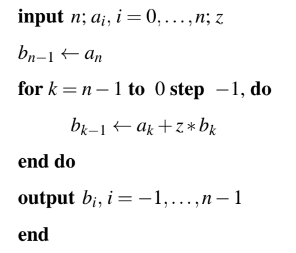
\includegraphics[width=0.34\linewidth]{horner.png}};
        \end{tikzpicture}
    }


    \column{0.5}
    \block{Ventajas}{
        \begin{itemize}
            \item Reduce la cantidad de operaciones necesarias para evaluar un polinomio.
            \item Es más eficiente que el método usual.
            \item Es más fácil de programar.
        \end{itemize}
    }

    \block{Implementación en Python}{
        En python el código para evaluar un polinomio en un valor específico de $x$ es el siguiente:	
        \begin{tikzfigure}[Algoritmo de Horner Python.]
            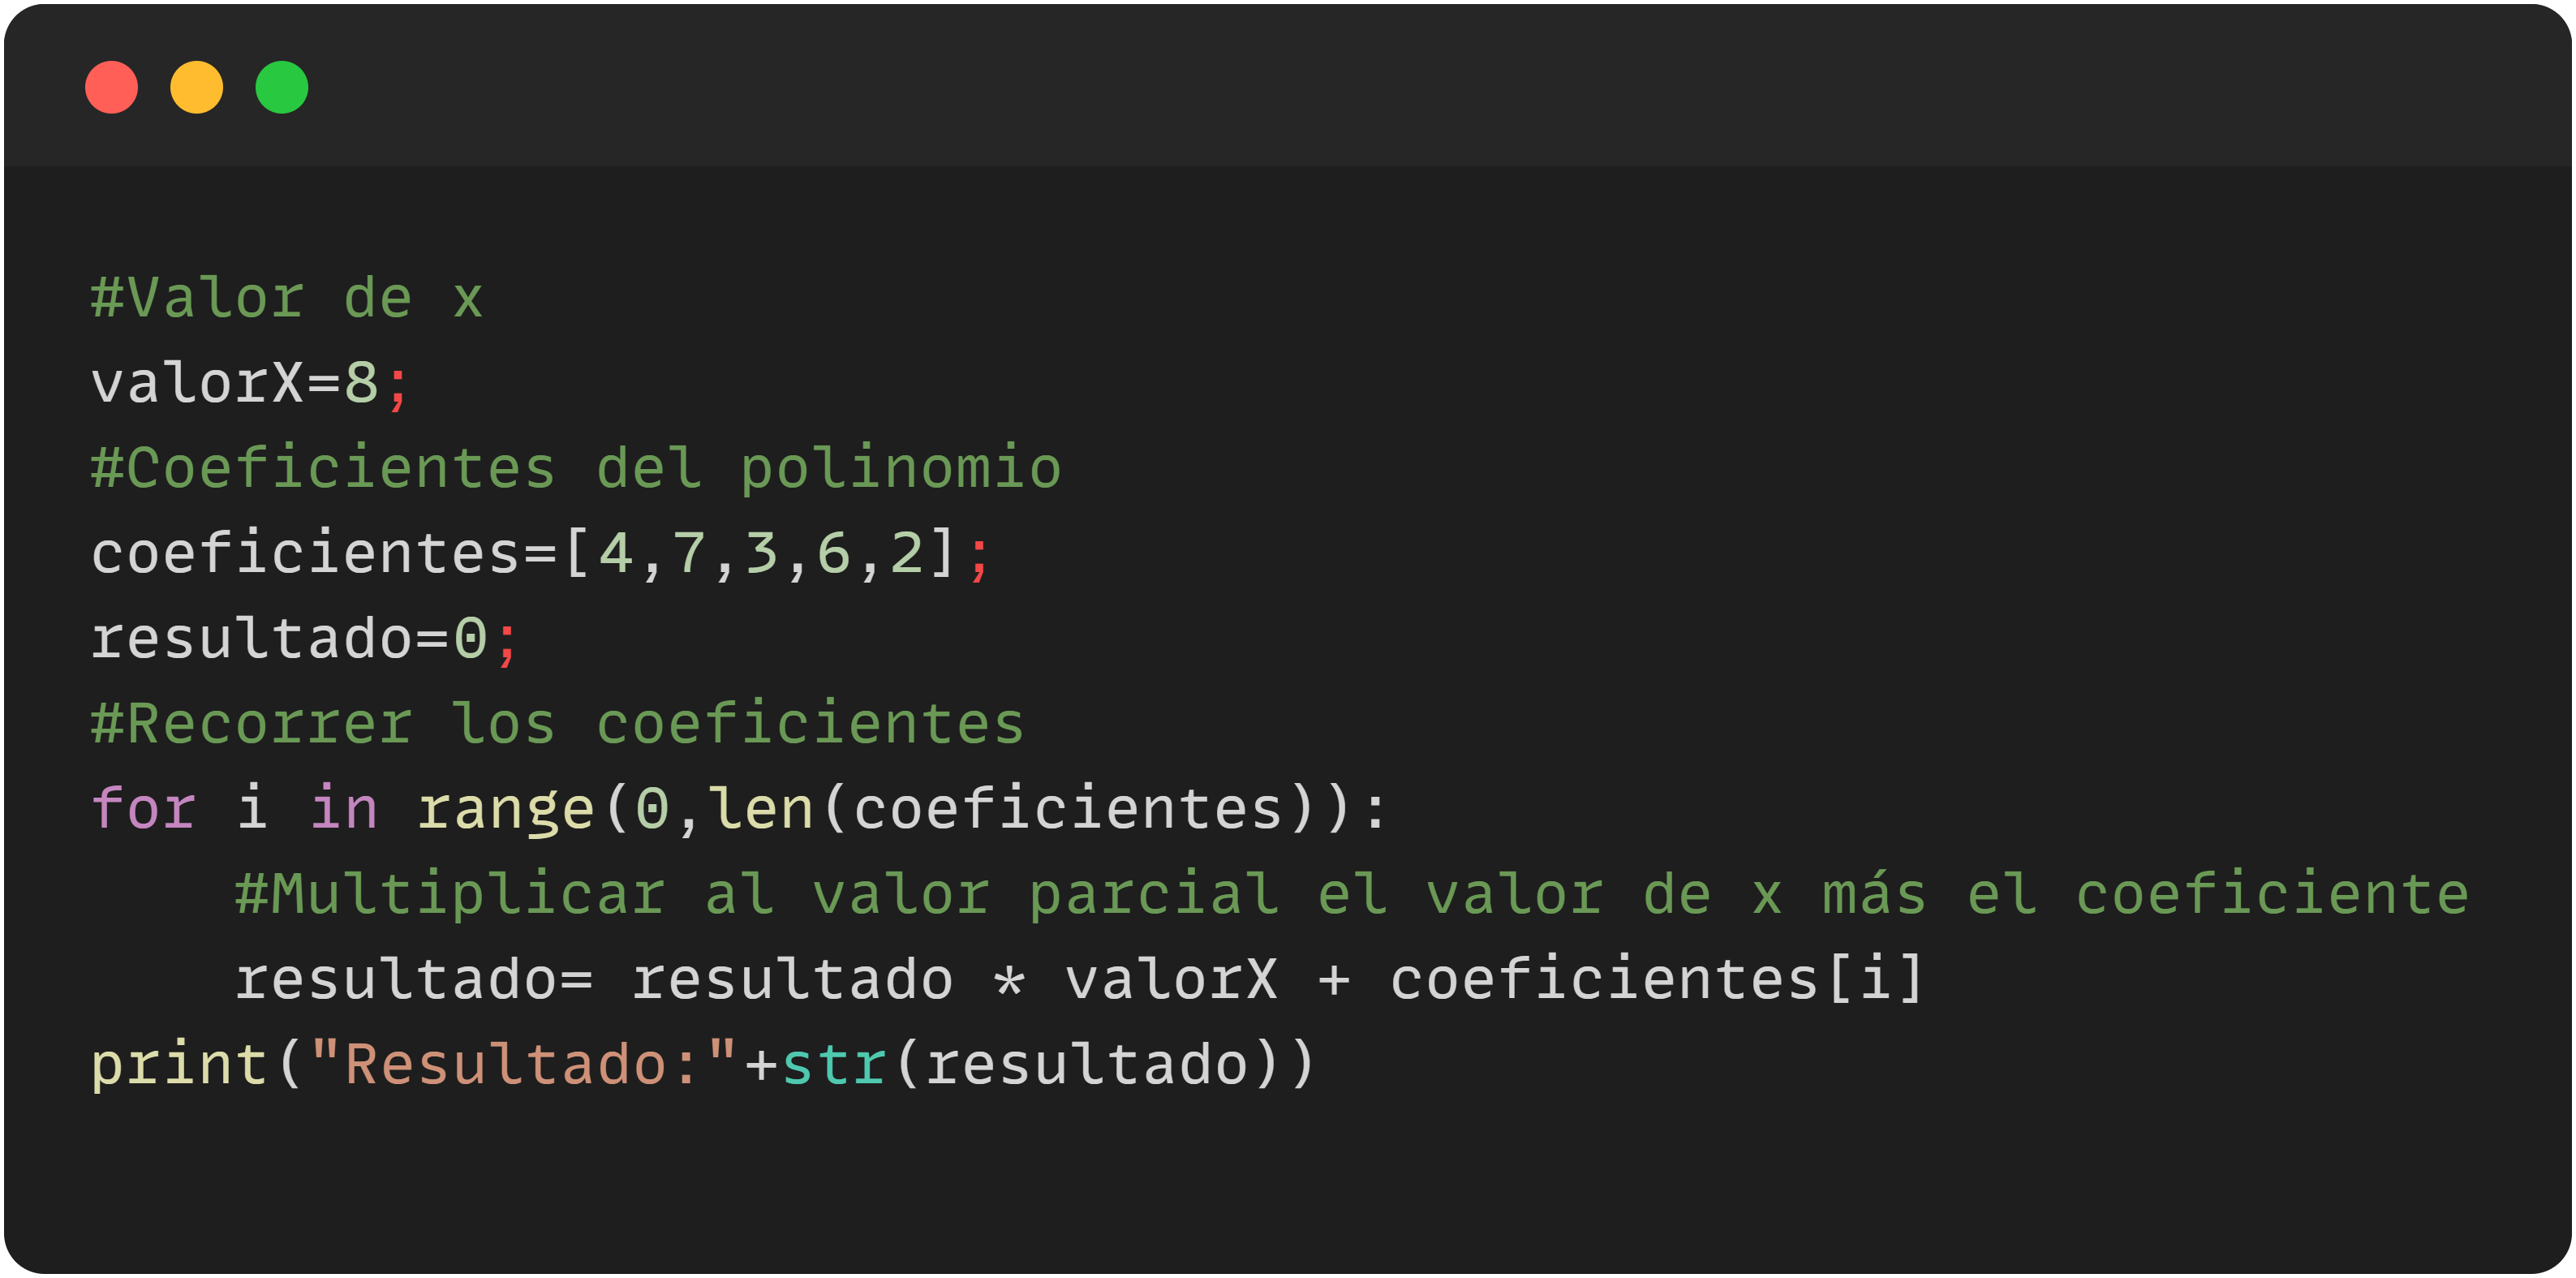
\includegraphics[width=0.5\linewidth]{horner-python.png}
        \end{tikzfigure}
    }

    \block{Implementación en C}{
        En C el código para evaluar un polinomio en un valor específico de $x$ es el siguiente:	
        \begin{tikzfigure}[Algoritmo de Horner C.]
            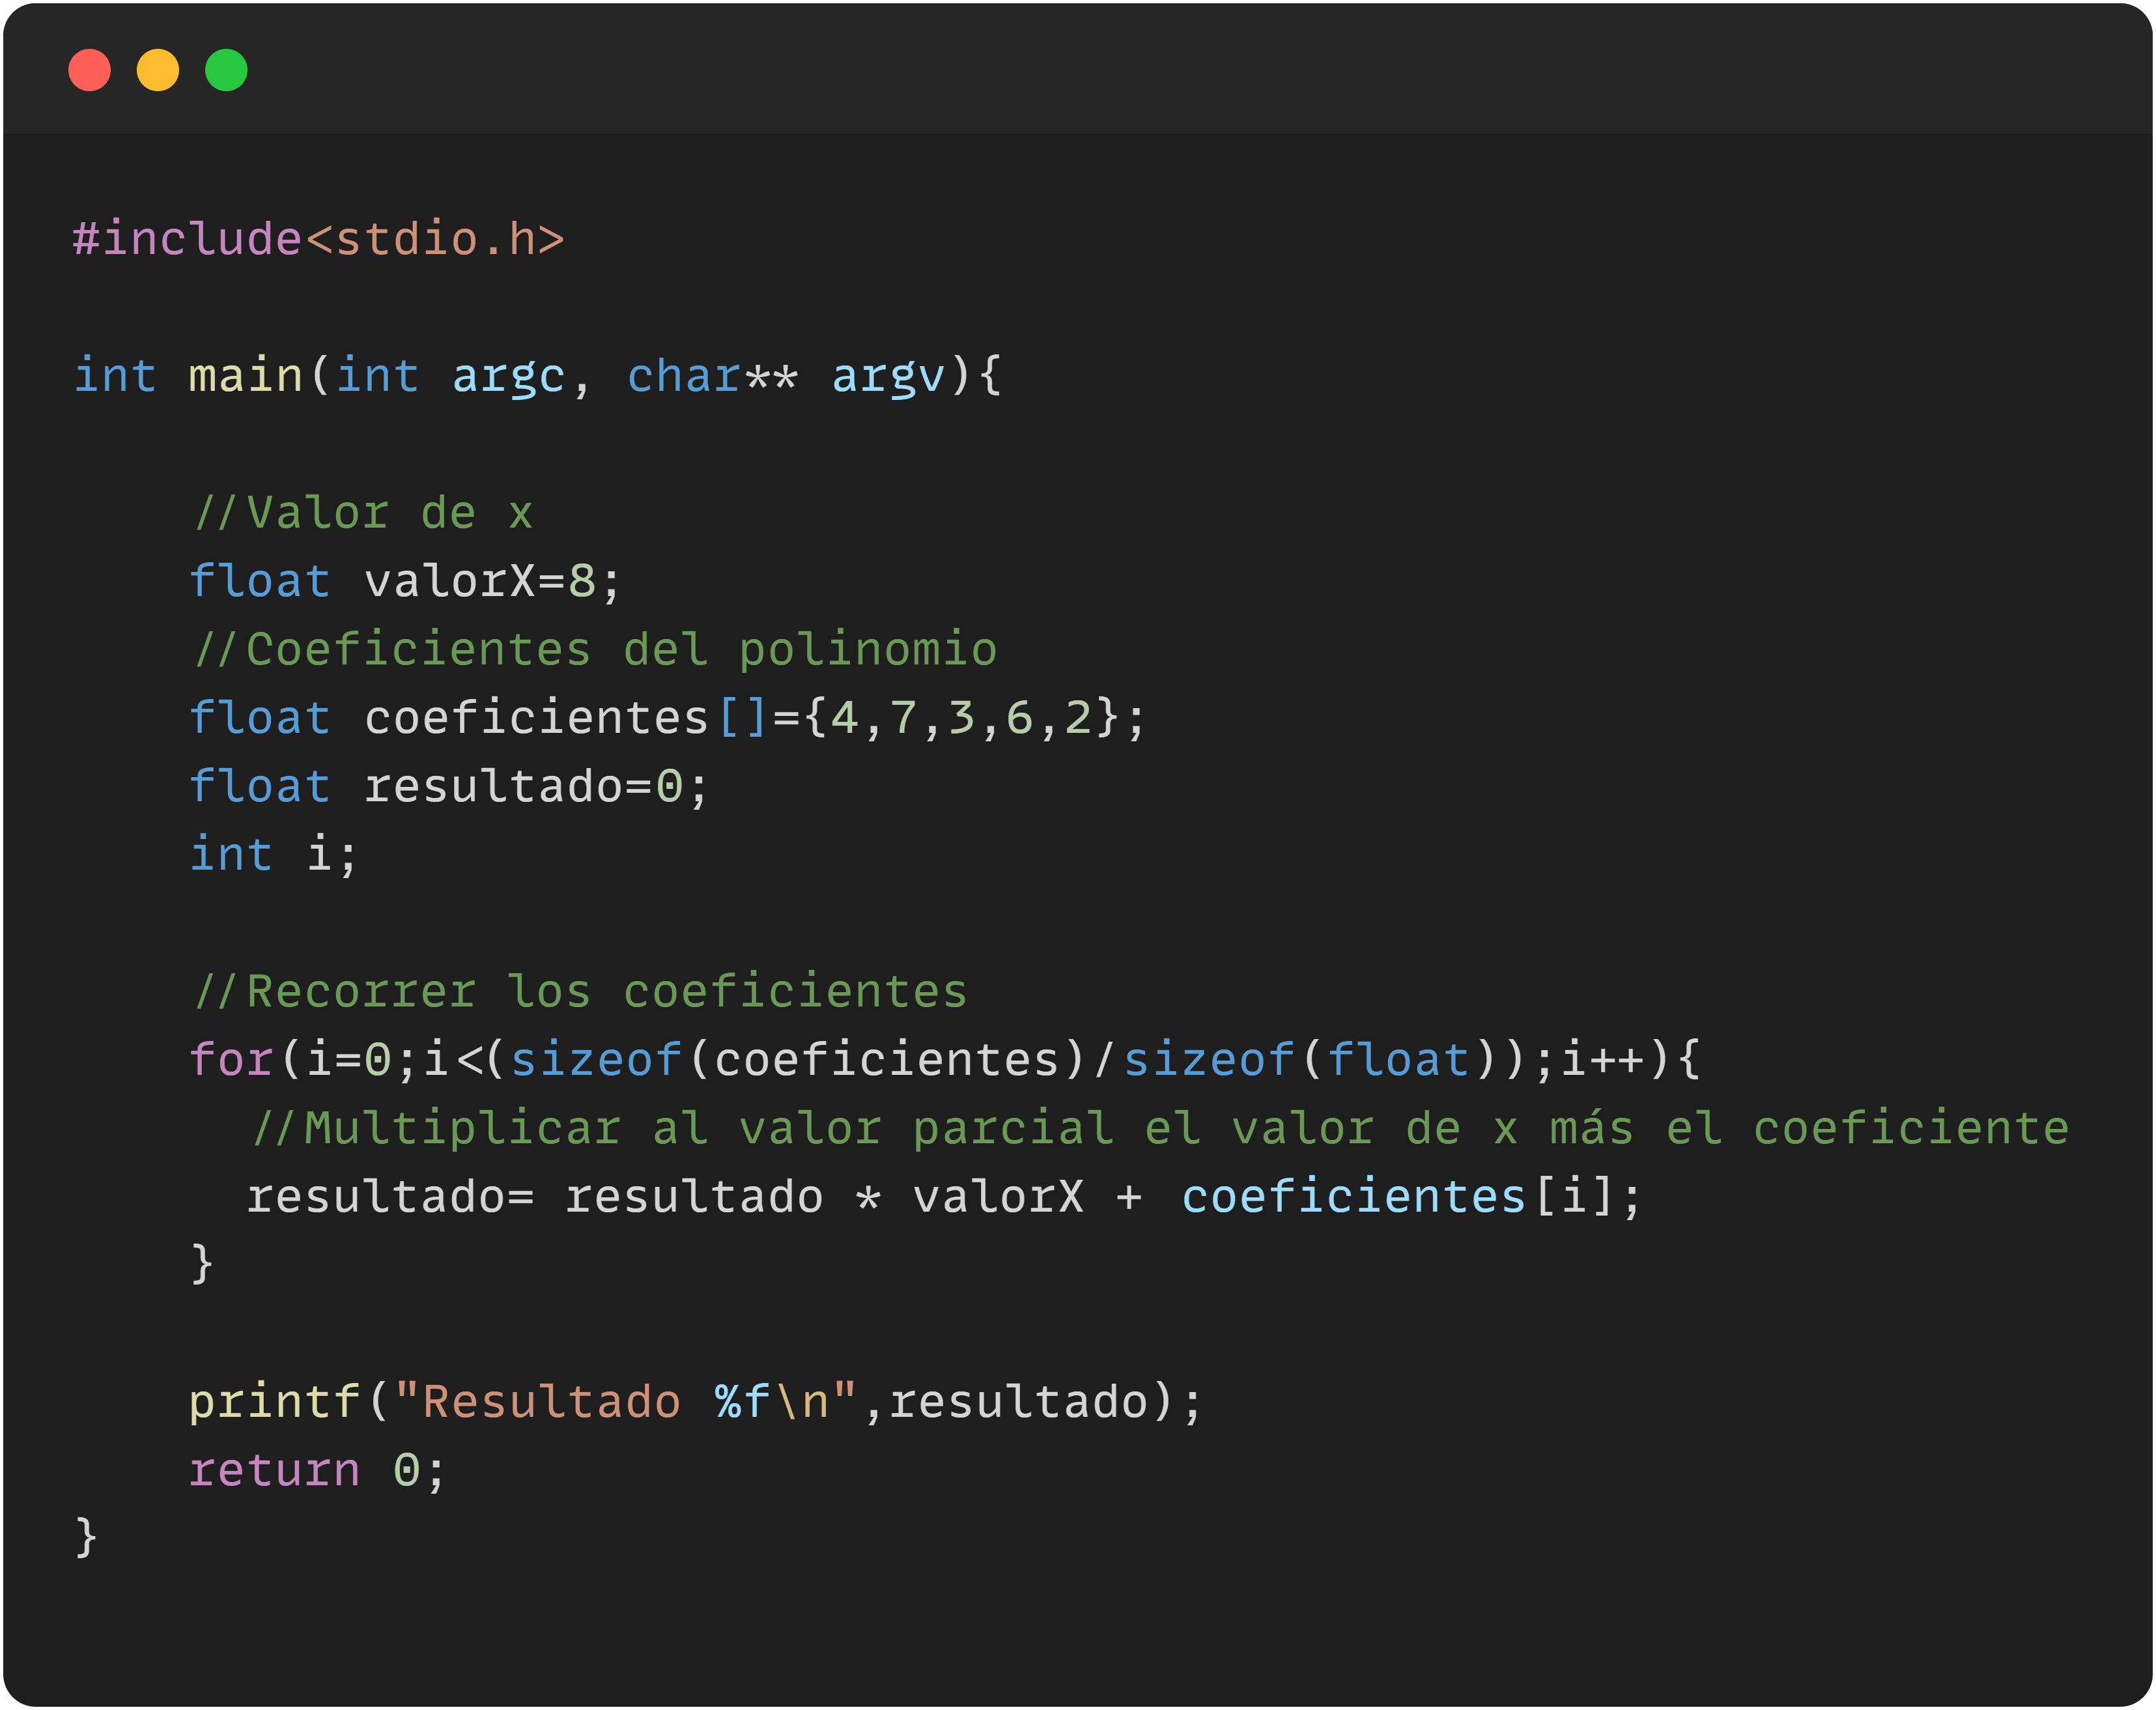
\includegraphics[width=0.5\linewidth]{horner-c.png}
        \end{tikzfigure}
    }
        
}

\end{columns}

\end{document}